% 调用上级目录公共模板
\documentclass{../template/softeng}

\begin{document}

% 封面：文档名、项目名、版本
\doccover{软件需求规格说明书}
{在线论文文档自动生成系统}
{V2026.07}

% 目录
\tableofcontents
\newpage

% 修订记录
\begin{revrecord}
V1.0 & 2026-07-10 & 郑羽婷 & 陆思雨 & 初稿完成，完成功能性需求 \\
\hline
V1.1 & 2026-07-11 & 陆思雨 & 李四 & 对目标和功能描述进行调整修改 \\
\hline
\end{revrecord}

% 正文正文结构（软件工程国标标准章节）
\section{引言}
\subsection{编写目的}
本文档为在线论文文档自动生成工具软件需求规格说明书，用于完整定义系统全部功能性与非功能性需求，明确项目开发边界、业务规则、数据规范、运行约束。
本文档交付对象包含项目经理、系统设计人员、前后端开发工程师、测试人员，作为项目规划、架构设计、代码开发、功能测试、验收交付的核心依据。

\subsection{项目背景}
本系统为高校大二软件工程实训项目，开发单位为在校实训开发小组，服务对象为高校程序设计课程教师与在校学生。
系统独立部署运行，无第三方外部系统强制对接，仅依托Web服务、判题沙箱、数据库完成完整业务闭环，用于支撑线上编程练习、自动代码评测、学情统计与教学管理。

\subsection{定义}
\begin{itemize}
    \item JWT：JSON Web Token，用于前后端分离架构下的无状态身份鉴权工具；
    \item RBAC：基于角色的权限控制（Role-Based Access Control），通过用户-角色-权限的映射实现系统隔离；
    \item 富文本编辑器：网页端支持字体、层级、表格、图片嵌入的在线排版组件；
\end{itemize}

\subsection{参考资料}
\begin{enumerate}
    \item GB/T 9385-2008 计算机软件需求规格说明规范；
    \item GB/T 30998-2014 信息技术 用户界面 网页可访问性指南；
    \item 实训项目任务书：在线论文文档自动生成工具开发（2026软件工程实训）；
    \item 基于 JWT 的前后端分离无状态认证体系设计与安全规范；
    \item 基于 RBAC (基于角色的权限控制) 模型的多角色权限隔离设计指南[cite: 1]；
    \item MySQL 8.0 关系型数据库安全配置与高效索引设计手册[cite: 2]；
    \item 信息安全技术：Web 应用安全防护与防范水平/垂直越权技术规范。
\end{enumerate}

\section{任务概述}
\subsection{目标}
开发一套Web端在线论文编辑与标准化文档生成系统，主要用于辅助学生规范化完成课程论文、毕业论文、项目设计类论文的在线撰写、版式排版与文档导出。系统设置管理员、学生、教师三类用户角色，分别赋予模板管理、论文编辑导出、课程论文线上批阅等对应权限，实现论文模板统一配置、网页端图文表格参考文献编辑、全文在线预览、docx与PDF格式文件导出、课程论文批阅留痕等完整业务流程。。

\subsection{系统角色与权限划分}
基础架构必须在技术层面上强制约束并实现以下三类角色的权限边界：
\begin{itemize}
    \item \textbf{系统管理员}：具备系统后台基础数据管理、学院信息维护、多类型论文模板新增/编辑/上下架权限，安全策略上禁止其直接编辑学生论文内容。
    \item \textbf{学生用户}：具备选用模板、在线编辑论文、素材上传、草稿保存、全文预览、导出 Word/PDF 文档以及提交课程论文至教师端的权限。
    \item \textbf{教师用户}：仅针对课程论文拥有专属批阅权限，可执行查看内容、添加位置批注、填写评语、评定成绩、退回论文等操作，具备查看历次批阅历史记录的权限。
\end{itemize}

\subsection{运行环境}
\begin{itemize}
    \item 服务操作系统：Windows Server / Linux CentOS；
    \item Web服务：Nginx / Tomcat；
    \item 数据库：MySQL 8.0；
    \item 判题依赖：多语言编译器、隔离沙箱程序；
    \item 客户端：主流Chrome、Edge浏览器。
\end{itemize}

\subsection{条件与限制}
\begin{enumerate}
    \item 判题服务必须做代码隔离，禁止用户代码直接访问服务器本地文件；
    \item 系统需限制单用户单次代码运行时间、内存上限，避免服务器资源耗尽；
    \item 仅支持教师、学生两种角色，不开放游客完整答题权限；
    \item 题库批量导入仅支持标准格式化文本文件，不支持自定义复杂格式；
    \item 平台部署硬件资源有限，并发判题任务数量存在上限。
\end{enumerate}

\section{数据描述}
\subsection{静态数据}
系统长期持久存储的不变基础数据：用户账号信息、角色定义、权限节点、学院/院系基础信息表。
\subsection{动态数据}
系统运行过程中实时产生、变更的数据：用户登录 Token 会话、论文草稿、参考文献条目、教师批注与评分记录、版本流转历史日志。

\subsection{数据库介绍}
采用 MySQL 8.0 关系型数据库体系，由基础架构人员统一设计并建立以下核心鉴权及基础信息表，各表通过外键或关联字段建立物理/逻辑约束：
\begin{itemize}
    \item \textbf{用户表 (sys\_user)}：存储用户唯一标识 (UID)、用户名、加盐哈希密码、所属学院 ID、账号激活状态、创建时间等。
    \item \textbf{角色表 (sys\_role)}：存储固定三类角色（ADMIN, STUDENT, TEACHER）的标识与描述。
    \item \textbf{用户角色关联表 (sys\_user\_role)}：维护用户与角色的多对多/一对一映射关系，作为后端鉴权拦截的直接依据。
    \item \textbf{学院信息表 (sys\_college)}：维护全院系的基础数据，供管理员维护及学生选用模板时进行维度筛选。
\end{itemize}
\subsection{数据词典}
包含用户ID、用户名、角色标识、题目ID、难度等级、输入输出样例、时间限制、内存限制、提交状态码、判题耗时、通过率、在线人数、队列长度等全部字段含义、数据类型、取值范围说明。

\subsection{数据采集}
\begin{itemize}
    \item 基础题库数据：教师手动录入或批量文件导入；
    \item 用户数据：学生注册、教师后台录入；
    \item 运行统计数据：系统后台定时采集在线、判题负载、提交数据；
    \item 交互数据：学生提交代码、发帖、评论行为实时采集入库。
\end{itemize}

\section{功能需求}
\subsection{功能划分}
系统基础架构划分为三大核心子模块：统一用户中心（注册/登录）、JWT 安全鉴权引擎、基于 RBAC 的多角色权限控制拦截器。

\subsection{功能描述}
\reqitem{FR001}{管理员可新增、编辑、删除学院信息，按学院维度对论文模板进行分类归属管理。}
\reqitem{FR002}{管理员可发布、编辑、启用、停用毕业论文、课程论文、项目论文等多类型模板，支持模板下架与版本管理。}
\reqitem{FR003}{管理员可配置模板内置章节结构，涵盖封面、原创声明、中英文摘要与关键词、多级章节正文、附录、参考文献等固定版式。}
\reqitem{FR004}{管理员可统一约束模板排版格式，包括字体、字号、行距、段落缩进、页边距、页眉页脚与页码等参数。}
\reqitem{FR005}{管理员可对模板进行在线预览与修改，模板更新后学生新建论文将自动套用最新版本。}
\reqitem{FR006}{学生可注册账号、登录系统、修改个人信息，按学院与论文类型筛选选用对应模板。}
\reqitem{FR007}{学生可依托模板大纲进行结构化章节编辑，支持标题层级设置、文字加粗、对齐方式、段落缩进等基础排版操作。}
\reqitem{FR008}{学生可从本地上传图片并嵌入文档指定位置，支持图片位置调整与大小修改。}
\reqitem{FR009}{学生可在线插入并编辑自定义表格，适配论文数据表格与学术三线表等使用场景。}
\reqitem{FR010}{学生可逐条录入参考文献的作者、标题、发表刊物、出版年份、页码等信息，系统按模板格式自动统一排版文献列表，并支持正文引用标注与文献条目关联。}
\reqitem{FR011}{学生编辑过程中系统自动保存草稿，同时支持手动保存，学生可多次进入系统查看、续写、修改历史论文文档。}
\reqitem{FR012}{学生可一键生成整篇论文的网页预览页面，完整展示封面、章节、图片、表格、参考文献的整体排版效果，支持分页浏览。}
\reqitem{FR013}{学生可按所选模板既定格式一键导出标准docx格式Word文档与PDF格式文件，导出内容排版规范、图文完整无错乱。}
\reqitem{FR014}{学生完成课程论文后可提交给对应授课教师，提交后文档锁定，仅教师可执行批阅或退回操作。}
\reqitem{FR015}{教师可在线查看学生提交的课程论文预览内容，在文档对应位置添加批注与修改建议。}
\reqitem{FR016}{教师可填写整体评语、评定论文分数与等级，也可退回论文供学生修改重提。}
\reqitem{FR017}{系统留存每一次提交、批阅、退回的版本记录，学生可查看全部批注内容并根据意见调整后重新提交复审。}
\reqitem{FR018}{系统对管理员、学生、教师三类角色进行身份认证与权限隔离，各角色仅可访问授权范围内的功能与数据。}

\section{性能需求}
\subsection{数据精确度}
判题结果严格匹配测试用例标准输出，无字符、空格、换行误差；统计通过率、解题数量数据精确至整数，排行榜实时数据无统计偏差。

\subsection{时间特性}
\begin{itemize}
    \item 网页页面加载响应时间 ≤ 1.5s；
    \item 普通代码提交判题反馈时间 ≤ 3s；
    \item 监控数据刷新间隔 5s；
    \item 批量导入题库处理单条题目耗时 ≤ 0.1s；
\end{itemize}

\subsection{适应性}
系统可适配Windows、Linux服务端环境；支持新增编程语言编译器；可扩展班级分组统计功能；可调整判题并发上限、代码运行时空限制参数。

\section{运行需求}
\subsection{用户界面}
采用Web网页可视化界面，题库分页列表、在线代码编辑器、监控数据图表、表格化提交记录、分页讨论帖子；统一菜单布局、按钮样式，弹窗提示操作结果。

\subsection{硬件接口}
无需专用硬件外设接口，仅依赖服务器CPU、内存、磁盘资源完成代码编译与数据存储。

\subsection{软件接口}
数据库接口：MySQL标准JDBC/ODBC连接接口；
判题接口：本地进程调用各语言编译器；
前端接口：前后端RESTful API数据交互接口。

\subsection{故障处理}
\begin{itemize}
    \item 数据库断开：页面提示服务器异常，缓存用户未提交代码；
    \item 判题服务器宕机：任务存入队列，恢复后自动重试判题；
    \item 超长恶意代码：直接拦截，返回运行超限错误；
    \item 文件上传失败：弹窗提示并保留本地代码。
\end{itemize}

\section{其它需求}
\begin{enumerate}
    \item \textbf{安全性}：系统内所有用户密码严禁明文存储，必须在后端采用强哈希算法（如 BCrypt 或 SHA-256 加盐）进行不可逆加密；传输层敏感接口需防范 SQL 注入攻击；JWT Token 需设置合理的过期时间（如 2 小时），并采用安全的密钥进行签名。
    \item \textbf{可维护性}：基础架构需集成标准日志框架（如 Logback/AOP 切面），自动记录用户登录、登出、论文提交、管理员模板下架等核心关键业务的审计日志，为后续系统运维提供追溯依据。
\end{enumerate}

% 插入图片示例（OJ系统用例图）
\begin{figure}[htbp]
    \centering
    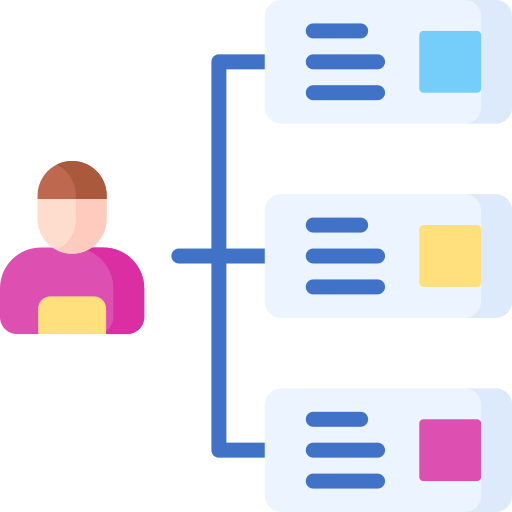
\includegraphics[width=0.7\textwidth]{usecase.png}
    \caption{在线OJ系统整体用例图}
\end{figure}

% 代码块示例（简易判题结果状态枚举）
\begin{lstlisting}[language=Python]
# 判题结果状态枚举
class JudgeStatus:
    ACCEPT = "AC"          # 通过
    WRONG_ANSWER = "WA"    # 答案错误
    COMPILE_ERROR = "CE"   # 编译错误
    TIME_LIMIT = "TLE"     # 超时
    MEMORY_LIMIT = "MLE"   # 内存超限
    RUNTIME_ERROR = "RE"   # 运行时错误
\end{lstlisting}

\end{document}